%\documentclass[a4paper]{fhnwreport} %Legt grundlegende Formatierungen wie Schriftarten, Ort Seitenzahlen etc. fest.
%
%\graphicspath{{./graphics/}}%Change according to graphics folder!
%
%\begin{document}

\section{Software}
Die Anforderung des Auftraggebers beinhaltet, dass die Kommunikation zwischen Sensorplatine und Meldezentrale über die Powerline erfolgt und keine zusätzliche Leitung beanspruchen darf. Für die drahtlose Übertragung war die Idee die Kommunikation über ein kabelloses System, wie Bluetooth oder Wireless zu verwenden. Diese Idee wurde aufgrund der unbekannten Distanzen zwischen der Sensor- und Meldeplatine verworfen. Die Kommunikation über die Powerline verlangt, dass die zu übertragenden Daten im richtigen Format in die Leitung eingekoppelt werden. Für diese Einkopplung wird ein fertiger Transceiver und ein Kommunikationsprotokoll verwendet. Es wird auf der Sensorplatine ein Mikrocontroller ATMega328 verwendet. \todo{Kommt das nicht in den HW Teil?}


\subsubsection{Sensorplatine}
Die Aufgabe der Sensorplatine besteht aus der Verarbeitung der gemessenen Daten und der Übermittlung der Daten. In der Abbildung \ref{fig:Software_Flussdiagramm_Sensorplatine} ist der Verlauf dieser Verarbeitung ersichtlich.

\begin{figure}[htbp] 
  \centering
     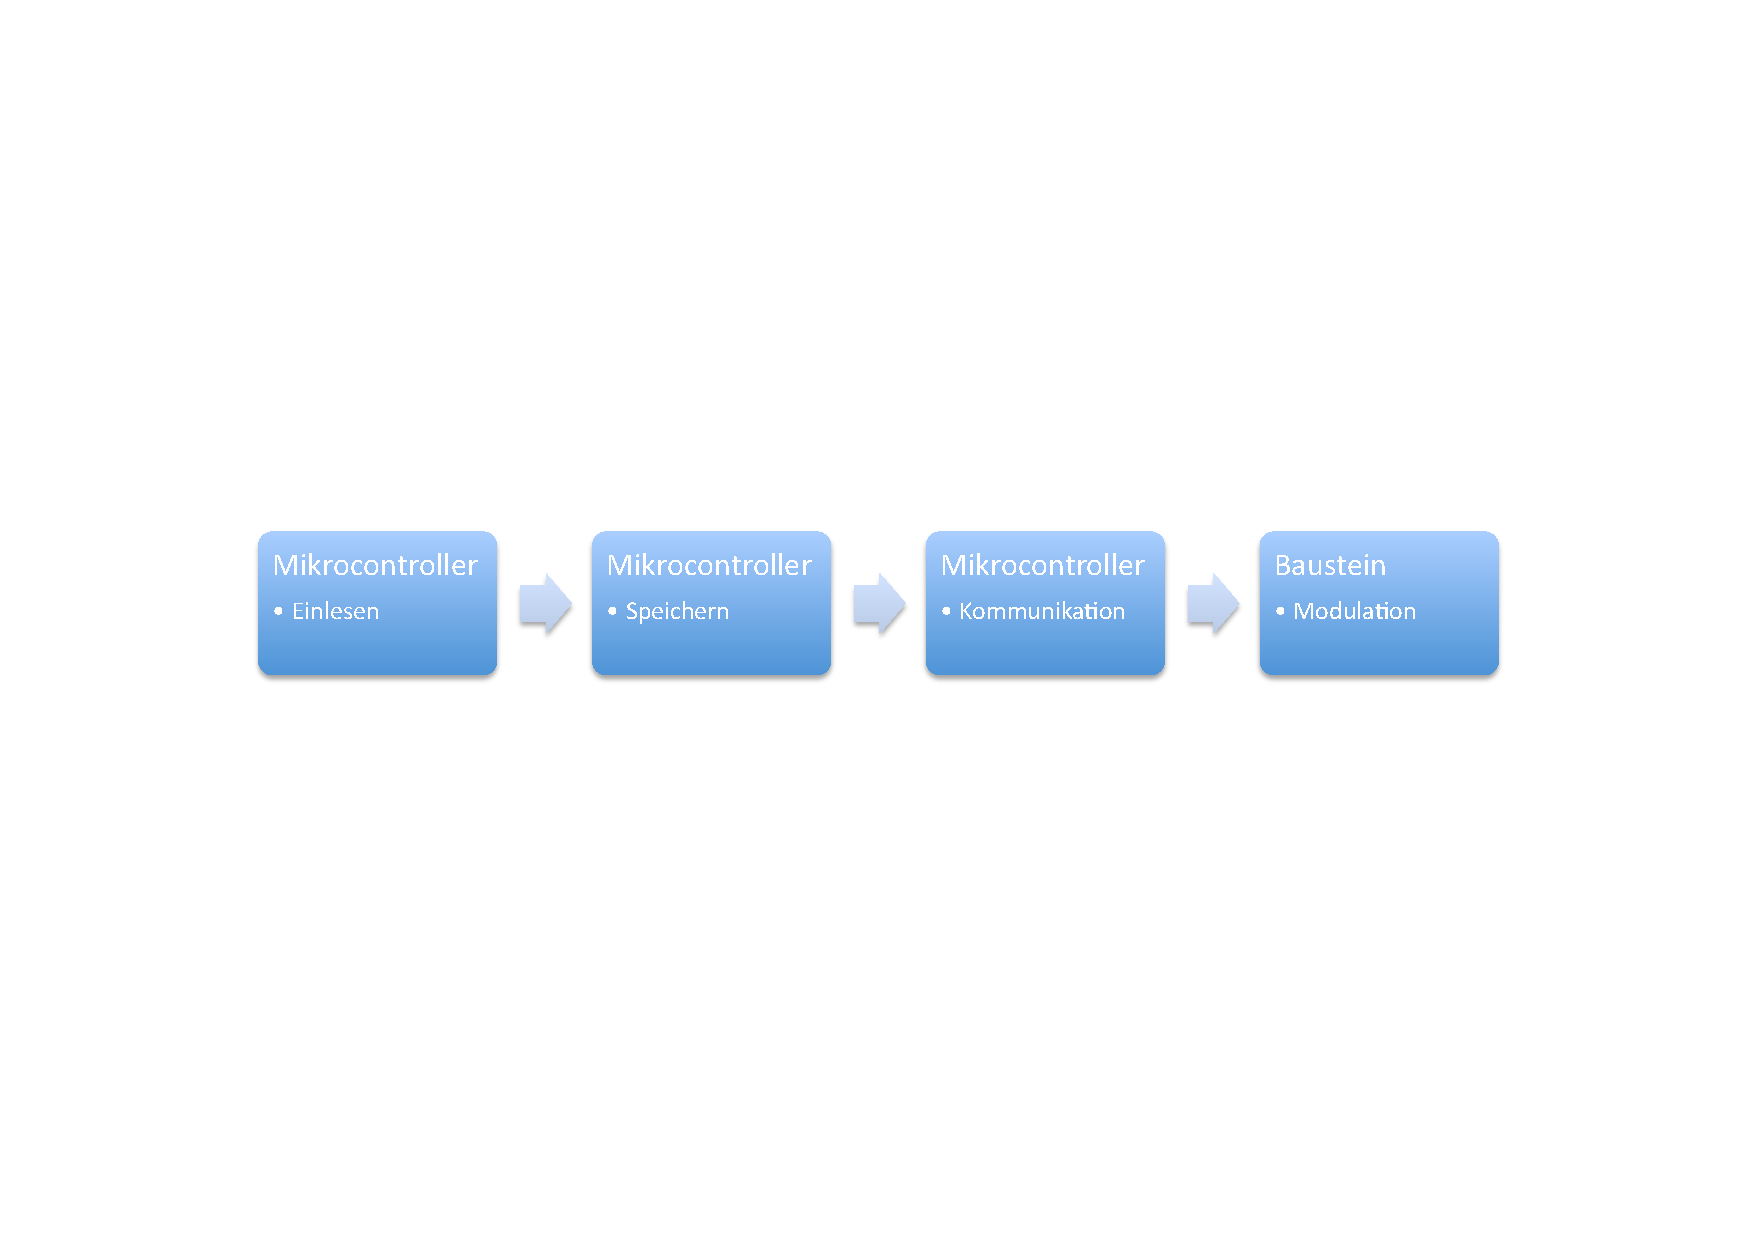
\includegraphics[width=1\textwidth]{graphics/Software_Flussdiagramm_Sensorplatine}
  \caption{Flussdiagramm Verlauf Programm Sensorplatine}
  \label{fig:Software_Flussdiagramm_Sensorplatine}
\end{figure}

Im ersten Schritt in der Abbildung \ref{fig:Software_Flussdiagramm_Sensorplatine} werden von der Messung die Daten eingelesen und in verwendbare Datentypen gespeichert. Die Kommunikation zum Transceiver wird über eine serielle asynchrone Schnittstelle stattfinden. \\Der Modulator wird die Messdaten auf die Leitung, Powerline Communication, koppeln.

\subsubsection{Kontrollplatine}
Die Meldeplatine wird die Zentrale aller Sensorplatinen sein. Sie hat die Aufgabe den Betrieb der Anlage zu überwachen sowie die gesammelten und übermittelten Daten der Sensorplatinen auszuwerten. Für einen detektierten Fehler wird ein Relaiskontakt geschalten und die fehlerhafte Stelle auf dem Display eingeblendet. Der gesamte Verlauf ist in Abbildung \ref{fig:Scheme_report_board} dargestellt.

\begin{figure}[htbp] 
  \centering
     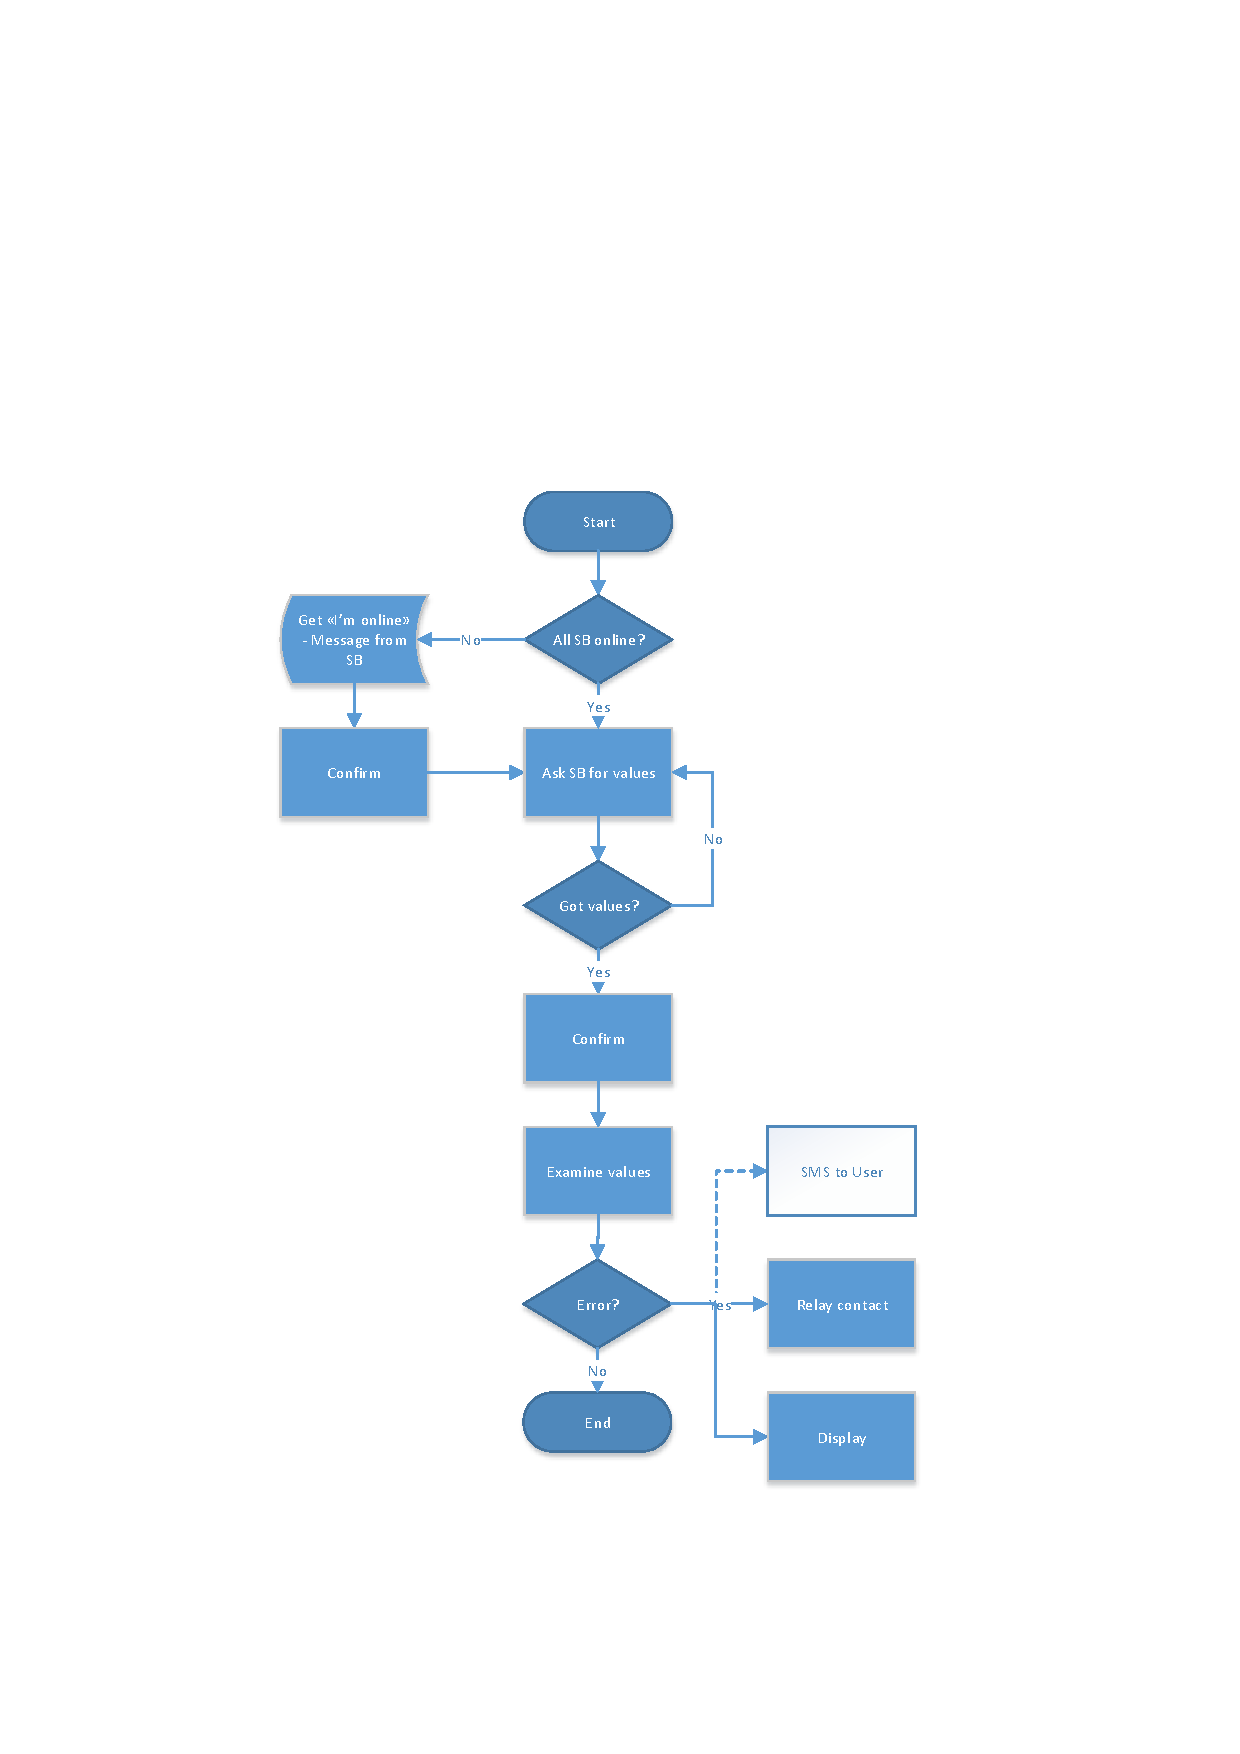
\includegraphics[width=1\textwidth]{graphics/Scheme_report_board}
  \caption{Flussdiagramm Verlauf Programm Meldeplatine}
  \label{fig:Scheme_report_board}
\end{figure}

Eine zuverlässige und ganzheitliche Überwachung der Anlage setzt die einwandfreie Kommunikation zwischen Sensorplatine und Meldeplatine voraus. Darum prüft die Meldeplatine als erstes die Verbindung (Abbildung \ref{fig:Scheme_report_board}: ``All Sensorboards online?'') zu den einzelnen Sensorplatinen. Die Meldeplatine wird dann die Abfrage der Messresultate geordnet koordinieren (``Ask Sensorboards for values'') und jeweils bestätigen. Im dritten Schritt wird die Menge an Messungen ausgewertet (``Examine values'') mit einem Algorithmus. Falls dann ein Fehler (``Error?'') detektiert wird schaltet ein Relaiskontakt ein externes Meldenetz. Zusätzlich wird der genaue Standort des Fehlers auf dem Display angezeigt.\\
Der Algorithmus für die Datenauswertung funktioniert nach dem arithemtischen Mittel. Es sagt aus, dass alle Datenpunkte addiert geteilt durch die Anzahl Datenpunkte einen Mittelwert ergibt. Entspricht ein einzelner Datenpunkt nicht dem Mittelwert ist dieser somit ein Fehler. Um anschliessend das fehlerhafte Modul zu lokalisieren bekommt jede Sensorplatine eine Identifikationsnummer, die alle in einem Anlagenschema hinterlegt sind.
%\end{document}